\chapter{List of tasks}
The following tasks is to be completed in the project:
\begin{enumerate}
	\item Improve hard iron calibration
	\item Implement accelerometer driver
	\item Tilt compensation
	\item Soft iron calibration
	\item Add gyroscope
	\item Dynamic calibration
	\item Final test
	\item Write report
\end{enumerate}

\section{Improve hard iron calibration}
It should be investigated if the current hard iron calibration is satisfactory, since it is rather simple in its current state. It currently take the average of the highest and lowest value measured for each component (x,y,z) and uses those three value as the hard iron offset. It might be better to use the mean for all points, center of gravity, center of mass, etc.

\section{Implement accelerometer driver}
To be able to determine the stationary pitch and roll angle of the device, the accelerometer will be used. This means a driver should be written to be able to utilize the accelerometer. The driver will be written in "C" and then bind to Lua. By binding the driver to Lua, the functions from the driver will importable in Lua.

\section{Tilt compensation}
The tilt compensation makes the device capable of measuring the magnetic field parallel to the surface of the earth with a pitch or roll angle. The tilt compensation will be done using the pitch and roll angle calculated from the accelerometer and the 3 components of measured magnetic field. 

\section{Soft iron calibration}
The soft iron calibration will make add soft iron distortion consideration to the calibration process. Soft iron distortions are caused by ferromagnetic material distorting the magnetic field depending on the direction of the magnetic field. The soft iron calibration is done by considering the measured magnetic field as a ellipse instead of a perfect circle. And by finding the major and minor axes of the ellipse it is then possible 

\section{Add gyroscope}
By adding a gyroscope to the device it will be possible to measure the rotation of the device. This will be necessary to implement a dynamic calibration of the device.

\section{Dynamic calibration}
The dynamic calibration is meant as a calibration where the device is rotating and moving while calibrating. So by utilizing both the accelerometer and the gyroscope it might be possible to do a dynamic calibration.

\section{Final test}
This is where the final testing of the final device will be done. This will involve the device being mounted to some kind of moveable configuration and the calibration results will be tested

\section{Write report}
This is where the report for the project will be written.

\begin{landscape}
	\chapter{Gantt chart}
	
	\begin{figure}[!h]
		\centering
		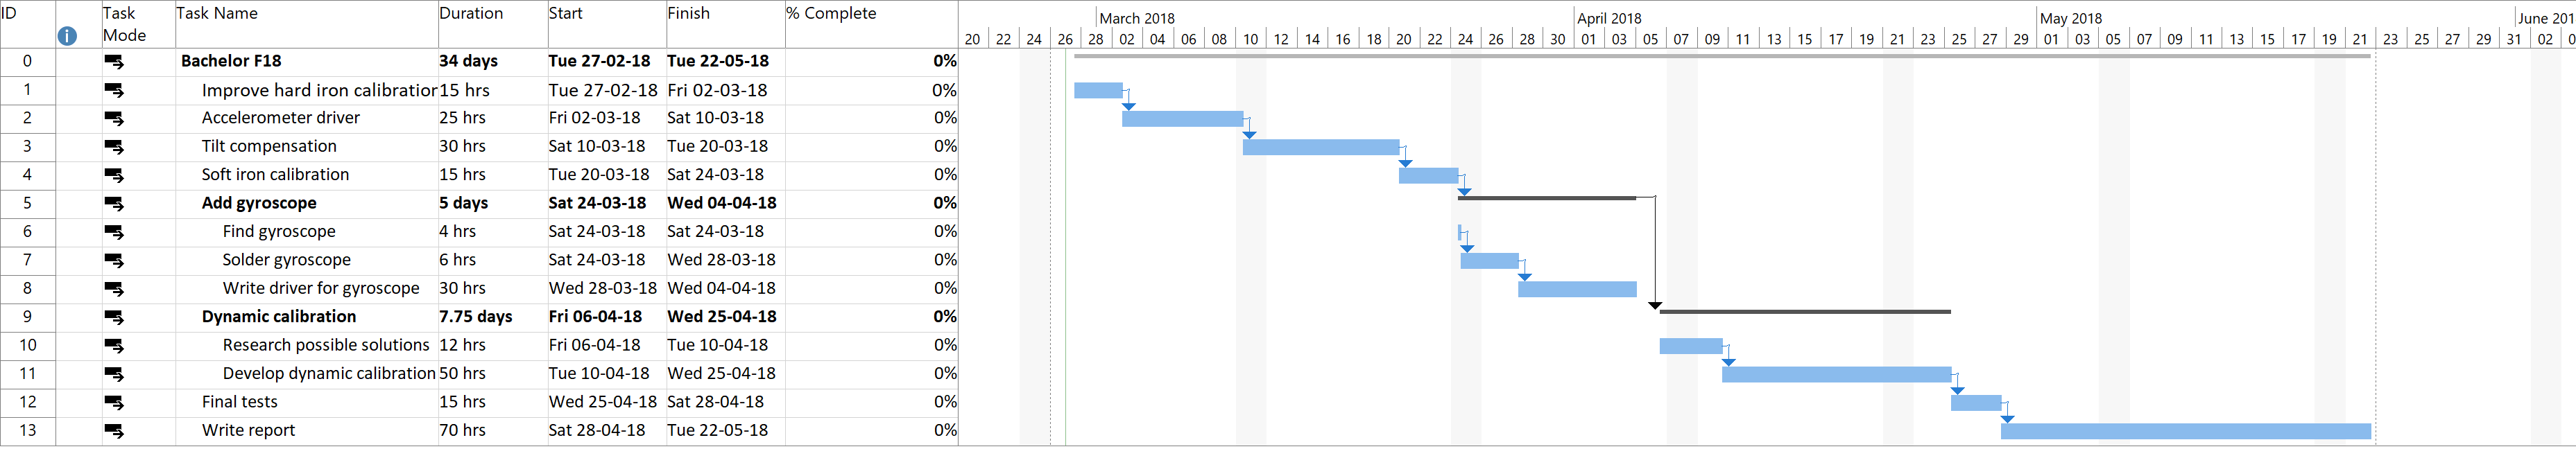
\includegraphics[width=1.4\textheight]{gantt.png}
		\caption{Gantt chart for the project with estimated hours per task}
		\label{fig:}
	\end{figure}

\end{landscape}
